\documentclass{article}

% Official NeurIPS template uses neurips_<year>.sty.
% This file prefers the official style when available and otherwise falls back
% to a close article layout so local builds do not break.
\newif\ifneuripsofficial
\neuripsofficialfalse
\IfFileExists{neurips_2026.sty}{
  \usepackage[final]{neurips_2026}
  \neuripsofficialtrue
}{
  \IfFileExists{neurips_2025.sty}{
    \usepackage[final]{neurips_2025}
    \neuripsofficialtrue
  }{
    \IfFileExists{neurips_2024.sty}{
      \usepackage[final]{neurips_2024}
      \neuripsofficialtrue
    }{
      \IfFileExists{neurips_2023.sty}{
        \usepackage[final]{neurips_2023}
        \neuripsofficialtrue
      }{
        \usepackage[margin=1in]{geometry}
      }
    }
  }
}

\usepackage[utf8]{inputenc}
\usepackage[T1]{fontenc}
\ifneuripsofficial\else
\usepackage{lmodern}
\fi
\usepackage{microtype}
\usepackage{amsmath,amssymb}
\usepackage{booktabs}
\usepackage{longtable}
\usepackage{float}
\usepackage{subcaption}
\usepackage{placeins}
\usepackage{graphicx}
\usepackage{xcolor}
\usepackage{hyperref}
\usepackage{url}
\usepackage{natbib}

\ifneuripsofficial\else
\hypersetup{
  colorlinks=true,
  linkcolor=blue,
  citecolor=teal,
  urlcolor=blue
}
\fi

\title{Uncertainty-Gated Safe RL with Quantum-Inspired Parameter-Efficient Estimation for Non-Stationary Control}

\author{Shivang Gupta\\Indian Institute of Technology Roorkee}

\date{}

\begin{document}

\maketitle

\begin{abstract}
Safe RL systems usually fail when regime shifts are faster than policy adaptation. In governance-like control loops, that failure does not first appear as lower average reward; it appears as brittle decisions under uncertainty.

We study an uncertainty-gated safe RL controller that routes PPO actions through a calibrated uncertainty gate and a deterministic shield. The core contribution is a control architecture claim: uncertainty-gated routing plus deterministic shielding gives a better safety-stability operating point under shift than policy-only control, while a compact classically simulated VQC-style head serves as a parameter-efficient non-linear uncertainty estimator.

Our primary empirical evidence comes from standard constrained benchmarks (SafetyPoint\-Goal1-v0 and SafetyHalf\-Cheetah\-Velocity-v1; 30 seeds) plus 50-seed governance controller comparisons under matched protocols. Custom governance simulations are treated as stress tests, not as the sole source of external validity.

We also report a negative result directly: in one custom ablation workload, full-system reward (-1264.90) is below random (-1232.33). We keep this result because it clarifies what the method is and is not optimizing: the method improves control stability and safety-oriented behavior under shift, but does not guarantee reward dominance in every stylized reward design. The central claim is therefore parameter efficiency with comparable safety behavior rather than universal return superiority. In a separate larger-model efficiency protocol, the compact architecture achieves a 166.89$\times$ parameter reduction while remaining competitive on safety-oriented metrics.

Code and artifacts: \url{https://github.com/maverick0721/QAI-Chain.git}.
\end{abstract}

\section{Introduction}

A compact 6-qubit variational controller with uncertainty-gated routing improves hard-regime fallback precision (at intensity 1.0: 0.964 vs 0.743 for MC-dropout, with matched trigger rates) while preserving safety behavior in non-stationary governance dynamics.

The paper's primary claim is not ``quantum advantage'' and not universal reward dominance. The claim is architectural: in high-switch settings, uncertainty-gated routing and deterministic shielding produce more stable safety behavior than policy-only execution, and this can be implemented with a compact classically simulated uncertainty head.

Stated as a one-line contribution: we introduce and evaluate a deployable decision-time safety layer for safe RL under shift, where uncertainty-triggered branch selection and deterministic shielding jointly improve stability at constrained parameter budgets.

In decentralized governance, the painful failures are rarely about average reward. They show up when load shifts quickly, latency spikes, and attack pressure distorts telemetry. The practical question is whether a controller stays predictable when estimates are noisy and the regime changes mid-episode.

QAI-Chain was built to study that exact failure mode. The empirical focus is narrow and operational: once vanilla PPO is placed in adversarial, regime-switching dynamics, can uncertainty-gated safe control recover stability without sacrificing hard constraints?

For safety-critical RL practice, a practical pattern is uncertainty-gated fallback with deterministic post-checks. This pattern is not blockchain-specific and can transfer to other control domains where policy collapse is unacceptable.

The updated protocol gives three practical lessons. First, baseline reward alone is an incomplete indicator of safe behavior under shift. Second, deterministic heuristics remain strong in easier regimes and are not straw-man baselines. Third, once switching complexity rises, uncertainty-gated control preserves safety behavior with substantially fewer parameters, which is the paper's primary practical value.

Primary external evidence comes from standard constrained benchmarks (SafetyPointGoal1-v0 and SafetyHalfCheetahVelocity-v1, 30 seeds) and a matched 50-seed governance controller-comparison suite. Across these settings, reward-safety trade-offs remain compute-budget dependent.

Design-wise, we deliberately changed as little as possible. The controller keeps PPO's policy/value backbone and adds two controls: variance-aware reward shaping during training, and a decision-time routing rule that falls back to a resilience heuristic when uncertainty is high. In the complexity benchmark, only the risk weight $\lambda_{\mathrm{risk}}$ and uncertainty threshold $\tau$ are retuned across levels; model class and environment stay fixed. This keeps the comparison about efficient safety behavior, not architecture churn.

Deployment integrations (for example, on-chain audit commitments) provide optional provenance support in multi-party governance settings but are orthogonal to the core Safe RL mechanism evaluated in this paper.

\paragraph{Contributions.}
The paper makes the following contributions:
\begin{itemize}
    \item a decision-time safe-control architecture that combines uncertainty-gated fallback with deterministic shielding,
    \item a parameter-efficient uncertainty-estimation module (compact architecture) that preserves safety behavior under non-stationary disturbances,
    \item and a high-rigor evaluation protocol centered on completed 30-seed standard constrained-benchmark runs (SafetyPointGoal1-v0 and SafetyHalfCheetahVelocity-v1), with a matched 50-seed governance controller-comparison suite and governance stress tests as supporting evidence.
\end{itemize}

\begin{table}[htbp]
\centering
\footnotesize
\setlength{\tabcolsep}{4pt}
\begin{tabular}{p{0.30\linewidth}p{0.30\linewidth}p{0.30\linewidth}}
\toprule
\textbf{Safety Mechanism} & \textbf{Efficiency Mechanism} & \textbf{Audit Mechanism} \\
\midrule
Uncertainty-gated routing plus deterministic shielding enforces safe execution under regime shifts. & A compact uncertainty head reduces parameter count while preserving control quality. & Optional tamper-evident commitments support governance traceability. \\
\midrule
Primary algorithmic claim. & Secondary efficiency mechanism. & Deployment layer; not required for core Safe RL results. \\
\bottomrule
\end{tabular}

\caption{Core contribution layering: what is algorithmically novel versus efficiency support versus deployment engineering.}
\label{tab:core-contribution-layers}
\end{table}

\paragraph{Scope.}
The empirical claim is specific and testable: uncertainty-gated control with compact architecture achieves comparable safety behavior at materially lower parameter budget under non-stationary governance dynamics, and this can be measured with fixed-seed paired comparisons \citep{dror2018hitchhikers,pineau2021improving,wilson2017good}.

\section{Related Perspectives}

Blockchain and ML integration work often focuses on transaction analytics, mechanism optimization, or fraud detection in mostly stationary settings. Governance control with adversarial perturbations has received less systematic, reproducible treatment. Classical consensus foundations remain essential \citep{nakamoto2008bitcoin}, and PPO remains a practical baseline for continuous-control policy learning \citep{schulman2017ppo}, but both need stress-tested evaluation when used in operational control loops.

Safe RL literature offers several tools with different assumptions: CVaR objectives \citep{chow2015cvar}, robust MDP formulations \citep{iyengar2005robust}, and constrained policy optimization \citep{achiam2017cpo}. Recent practice also emphasizes distribution-shift robustness, risk-sensitive policy updates, and uncertainty-aware action filtering. The approach here keeps PPO as the optimizer and adds uncertainty-aware routing at action time with risk shaping during updates. We evaluate this controller pattern against strong heuristic and constrained baselines under the same disturbance model, and we explicitly treat this paper as a systems-and-control contribution rather than a new policy-optimization objective.

Relative to modern safe-RL directions (risk-sensitive updates, uncertainty-aware filtering, and robust constrained control), this work contributes primarily at the control-architecture layer: it specifies how to combine branch-level uncertainty routing with deterministic post-check execution in a reproducible deployment pipeline. Expanding direct head-to-head comparison against additional recent baselines is an explicit next step, not an omitted assumption.

Reproducibility details are provided in dedicated checklist material, while the main text focuses on algorithmic behavior and safety-relevant outcomes.

\section{System Design}

Draw the runtime on a napkin and it is linear: telemetry in, policy guesses, maybe the gate vetoes, the shield always edits last, actuators see something bounded. Chain commits ride afterward if you want receipts two companies can argue over later.

\[
\text{state telemetry} \rightarrow \text{policy proposal} \rightarrow \text{uncertainty gate} \rightarrow \text{shield} \rightarrow \text{executed action}.
\]

Learning stays in Python/Sim; hashes land once the action is final so nobody pretends the ledger is on the hot gradient path.

\subsection{System Diagram}

\begin{figure}[H]
\centering
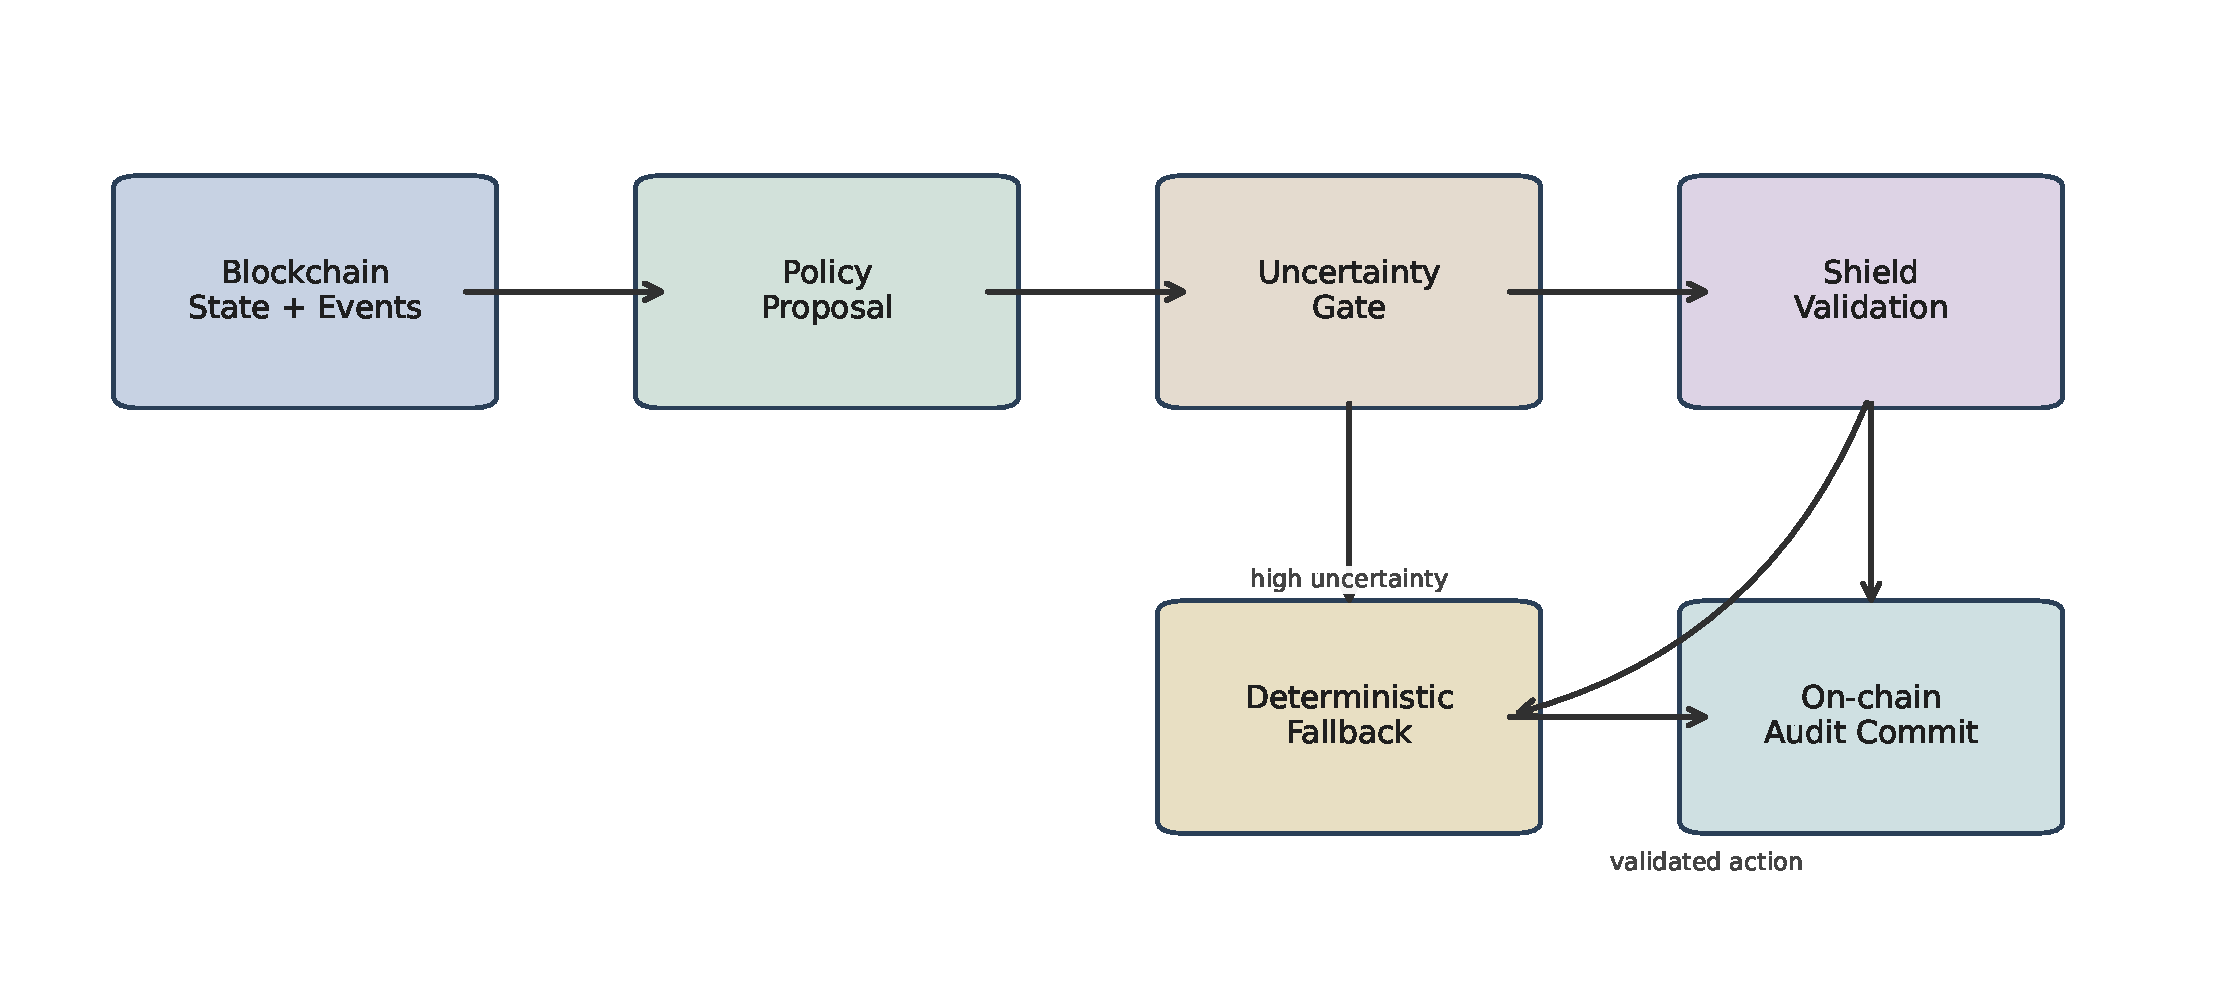
\includegraphics[width=0.95\linewidth]{figures/architecture_flow.pdf}
\caption{Runtime sketch: policy, gate, shield, optional commit.}
\label{fig:system-mermaid-rendered}
\end{figure}

\subsection{Data and Control Flow}

Peers and txs move ledger state through RPC plus validation. The controller ingests a compressed governance vector and proposes bounded knobs---difficulty, block size, gas limit. Same story as the napkin, typeset with the shield explicit:

\begin{equation}
\begin{aligned}
\text{State telemetry} &\rightarrow \text{policy proposal} \rightarrow \text{uncertainty gate} \\
&\rightarrow \text{safety shield} \rightarrow \text{on-chain commit}.
\end{aligned}
\end{equation}

Gate can punt to a heuristic first; shield can clamp or reject anyway. Every number in the paper assumes that gated-then-shielded path. Receipt/Merkle minutiae sit in appendix text if you need them.

\subsection{API Contracts}

RPC structs are typed; junk input throws instead of silently widening what the adaptive layer may try. Negative-path tests on malformed fields are boring and necessary.

\subsection{Operational Guardrails}

Typed interfaces, those tests, and a fixed ordering between policy, gate, and shield keep multi-node runs from decaying into ``works on my laptop.'' Zero novelty medals; it is what keeps pages legible when pagerduty fires at 2\,am.

\section{Methodology}

\subsection{Control Objective}

Reward mashes throughput, latency-shaped terms, a decentralization proxy, and distance to a moving target:
\[
\begin{aligned}
r ={}& w_1 \cdot \text{throughput} + w_2 \cdot \text{latency}(d) \\
&+ w_3 \cdot \text{decentralization} - \lambda |d - d_t|.
\end{aligned}
\]
Shield always sees actions after clipping.

\subsection{Policy Family}

Controllers span random, hand-tuned heuristics, vanilla PPO-family runs, and the robust gated recipe. PPO stays clipped \cite{schulman2017ppo}; our robust branch subtracts rolling reward variance:
\[
\tilde r_t = r_t - \lambda_{\mathrm{risk}}\,\mathrm{Var}(r_{t-k:t}).
\]

\subsection{Shield Logic (Executable Rule)}

Shield code is deterministic, state-aware, and boring on purpose---box constraints plus a per-step slew cap before anything executes:
\[
a^{\mathrm{exec}}_t=\mathrm{clip}(a_t, a_{\min}, a_{\max}),
\]
\[
\Delta a_t=\mathrm{clip}(a^{\mathrm{exec}}_t-a_{t-1},-\delta_{\max},\delta_{\max}).
\]
Still unsafe on a predicate (delay projection, partition threshold, etc.)? Swap to heuristic $a_t^{\mathrm{heur}}$ and re-run the checks. Code-level sketch:
\begin{itemize}
    \item If \texttt{hard\_safe(state, action)} is false, clamp action by bounds and max delta.
    \item Re-check safety; if still false, switch to \texttt{heuristic\_action(state)}.
    \item Return the validated action.
\end{itemize}

For explicit auditability, shield execution is summarized below:
\begin{enumerate}
    \item Input $(s_t, a_t, a_{t-1})$.
    \item Set $a\leftarrow\mathrm{clip}(a_t,a_{\min},a_{\max})$.
    \item Set $a\leftarrow a_{t-1}+\mathrm{clip}(a-a_{t-1},-\delta_{\max},\delta_{\max})$.
    \item If $\mathrm{hard\_safe}(s_t,a)$, return $a$.
    \item Set $a_h\leftarrow\mathrm{heuristic\_action}(s_t)$.
    \item Set $a_h\leftarrow\mathrm{clip}(a_h,a_{\min},a_{\max})$.
    \item Set $a_h\leftarrow a_{t-1}+\mathrm{clip}(a_h-a_{t-1},-\delta_{\max},\delta_{\max})$.
    \item If $\mathrm{hard\_safe}(s_t,a_h)$, return $a_h$.
    \item Otherwise, return $\mathrm{emergency\_safe\_action}(s_t)$.
\end{enumerate}

\subsection{Quantum-Inspired Uncertainty Gate}

Front-end is a six-qubit variational sketch: angle embed, entangle, re-upload data, read Pauli-$Z$ for mean/scale-ish scalars. Uncertainty comes from shaking weights, not from mysticism:
\[
\begin{aligned}
u_q(x) &= \operatorname{Var}\left(\{\mu_{\theta+\epsilon_k}(x)\}_{k=1}^{K}\right), \\
\epsilon_k &\sim \mathcal{N}(0,0.01I),\quad K=10.
\end{aligned}
\]
The routing rule is
\[
a_t=
\begin{cases}
a_t^{\mathrm{heur}}, & u_q(x_t)>\tau_q,\\
a_t^{\mathrm{policy}}, & u_q(x_t)\le\tau_q.
\end{cases}
\]

\subsection{Engineering Trade-offs in Uncertainty Design}

Offline pretty plots were not the bottleneck---serving cost was. Ensembles mean N forwards per step and N copies in RAM; perturbation keeps one net and jitters $\theta$ at inference, which is easier to colocate with a controller loop.

In our head-to-head grid the perturbation readout bought precision at fixed trigger budget versus MC-dropout and a small ensemble baseline without torching recall, so tuning targeted ``routing good enough at 10\% fire rate'' instead of chasing a single scalar uncertainty KPI.

\begin{figure}[H]
\centering
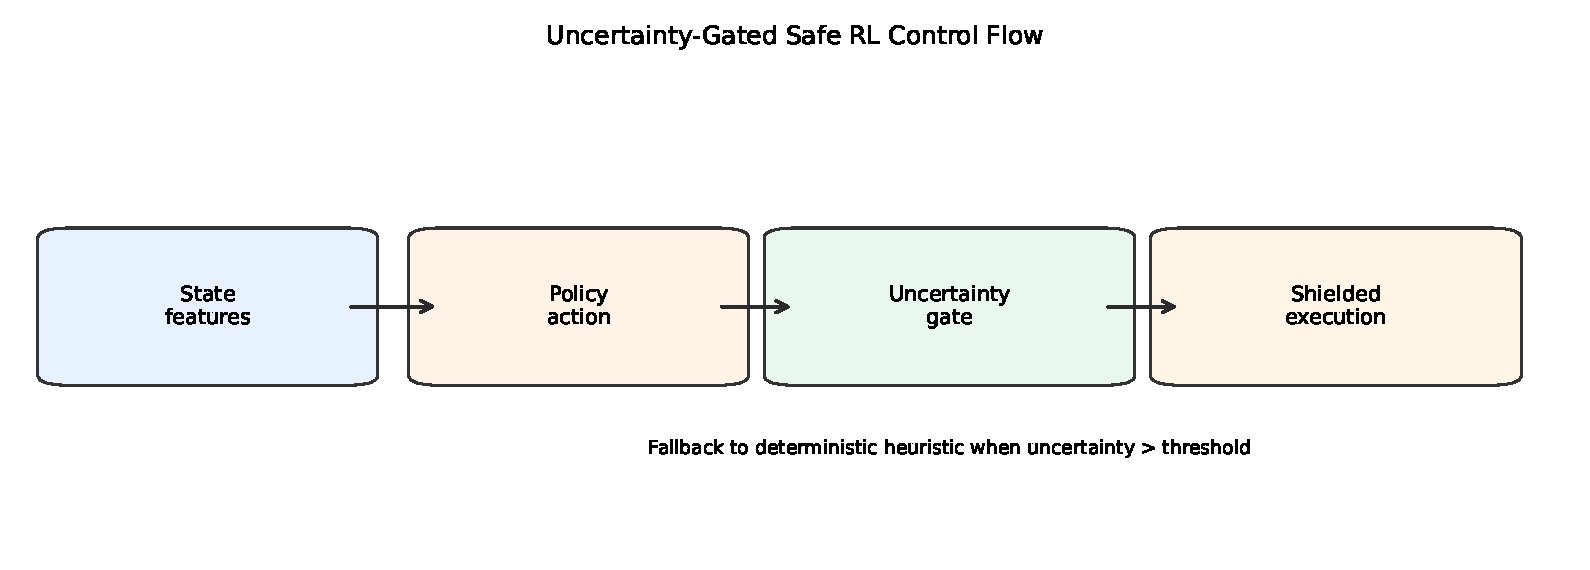
\includegraphics[width=0.88\linewidth]{figures/robust_policy_flow.pdf}
\caption{Fallback path: perturbation uncertainty $\rightarrow$ gate $\rightarrow$ shielded execution.}
\label{fig:robust-flow}
\end{figure}

\subsection{Why the Compact Estimator Compresses Well Here}

Classical simulation only; quantum throughput is irrelevant. Governance vectors in our build jam delay, congestion, attack pressure, and nasty cross-terms. Entangling layers mix multiplicatively on the cheap; re-uploading lets the same wires bend across time. Net effect: fewer weights than a fat MLP for the surface we needed. Compression only popped once gate+shield were live---without them the head trained on regimes it never had to stabilize.

\subsection{Adversarial and Ablation Design}

Scaled workload throws bursts, noisy delay, attack ramps, and regime hops. Seven toggles:
\begin{itemize}
    \item full system (quantum gate + shield + robust policy),
    \item no quantum gate,
    \item no shield,
    \item no fallback,
    \item classical PPO,
    \item Heuristic controller,
    \item random.
\end{itemize}
The stress-aware reward is
\[
\begin{aligned}
r_t^{\text{adv}} ={}& \alpha\,\text{throughput}_t - \beta\,\text{delay}_t - \gamma\,\text{attack}_t \\
&- \eta\,\text{fork}_t - \lambda |d_t-d^\star|.
\end{aligned}
\]

\subsection{Evaluation}

Scalars first: reward, violations, target MAE, fallback counters, a latency stand-in. Whenever two PPO-family rows get compared we bolt on bootstraps, permutation tests, and Cohen's $d$ so a single seed draw cannot ghost-write the conclusion \cite{efron1994introduction,good2005permutation}.
\section{Experimental Setup}

\paragraph{Protocol.}
Bucket~A stays deliberately dull: SafetyPointGoal1-v0 and SafetyHalfCheetahVelocity-v1, thirty seeds each, trained through official OmniSafe agents for CPO / P3O / PPOLag (no QAI-Chain gate or shield in that path---it is a sanity anchor that the repo and pinned deps reproduce standard constrained metrics). Bucket~B bruises harder---scaled governance (twelve states, three actions, two hundred steps, partial obs, injected telemetry faults) plus a toy DeFi loop (eight states, two actions, one fifty-step horizon, MEV and liquidity stress baked in), where the gate, shield, and robust stack evaluated in the paper actually run.

Tables pin seeds so pairwise comparisons do not wander when noise sneaks in. Heavy PPO-family and ablation grids use sixteen paired seeds; the constrained-baseline headline block uses fifty; uncertainty and efficiency cells use thirty so a single lucky draw cannot own the story.

\paragraph{Governance comparison method set.}
Controller grid: Random, Heuristic, CPO-style, P3O-style, PPO-Lagrangian-style, Robust QGate+Shield---same protocol in both custom environments.

\paragraph{Environment realism extension.}
Optional CSV traces drive demand, volatility, MEV-ish pressure, oracle noise so we can replay coarse historical shapes instead of only synthetic drift. The paper's trace-backed run feeds Ethereum daily gas prices (Etherscan) into intensity scheduling.

\paragraph{Primary Metrics.}
Means and standard deviations on reward, violation counts, target MAE, fallback counters, plus a per-step latency / forward-FLOPs proxy.

Fallback ticks whenever execution actually came from the deterministic branch---either the gate routed away from the policy or the shield vetoed the policy move and swapped in the heuristic.

\paragraph{Hypothesis Testing.}
Permutation tests plus effect sizes when PPO-family rows need pairwise structure; constrained suites compare final return, final cost, episode length directly. Bootstrapped 95\% intervals show up wherever bars read cleaner than lonely point estimates.

\paragraph{High-rigor constrained-baseline protocol.}
Fifty seeds, frozen knobs, metrics named before runs (reward, safety cost, hard-regime violations) so baseline ordering does not jitter on one seed lottery ticket.

\paragraph{Fair-capacity quantum-inspired efficiency protocol.}
VQC-28 beside MLP-28 beside a fatter MLP so ``different head'' does not silently mean ``different parameter budget.'' Raw counts and normalized views both land in the tables.

\paragraph{Primary standard-benchmark protocol.}
Safety Gym pair above, shared gating/shielding, three thousand steps per episode on the machine that generated Table~\ref{tab:standard-transfer-status}. Governance blocks stress regime behavior the Gym suites barely tickle.

\paragraph{Robust PPO settings.}
Risk-shaped rewards, quantum-uncertainty gate, contract-style shield. Perturbation batch uses $K{=}10$, Gaussian noise scale $0.01$ on weights. $\tau_q$ and $\lambda_{\mathrm{risk}}$ were tuned where switching gets aggressive.

\paragraph{Robust ablation variants.}
Seven toggles: Full (gate+shield+robust policy), No quantum gate, No shield, No fallback, Classical PPO, Heuristic, Random.

\section{Results}
\label{sec:results}

\subsection{Main Ablation Matrix}

\begin{table}[htbp]
\centering
\footnotesize
\setlength{\tabcolsep}{4pt}
\resizebox{\columnwidth}{!}{%
\begin{tabular}{lcccc}
\toprule
Configuration & Reward & Violations & Target MAE & Fallback Rate \\
\midrule
Full (QGate+Shield+Robust PPO) & -1264.90 & 55.31 & 3.372 & 0.000 \\
No Q-uncertainty gate & -1294.06 & 55.38 & 2.550 & 0.666 \\
No shield & -1287.71 & 55.31 & 4.063 & 0.000 \\
No fallback & -1287.71 & 55.31 & 4.063 & 0.000 \\
Classical PPO & -1284.05 & 55.31 & 2.763 & 0.000 \\
Heuristic & -859.22 & 53.19 & 2.832 & 0.000 \\
Random & -1232.33 & 55.25 & 3.628 & 0.000 \\
\bottomrule
\end{tabular}
}

\caption{Seven-configuration component ablation with side-by-side metrics (means from generated artifacts).}
\label{tab:component-necessity}
\end{table}

\begin{figure}[H]
\centering
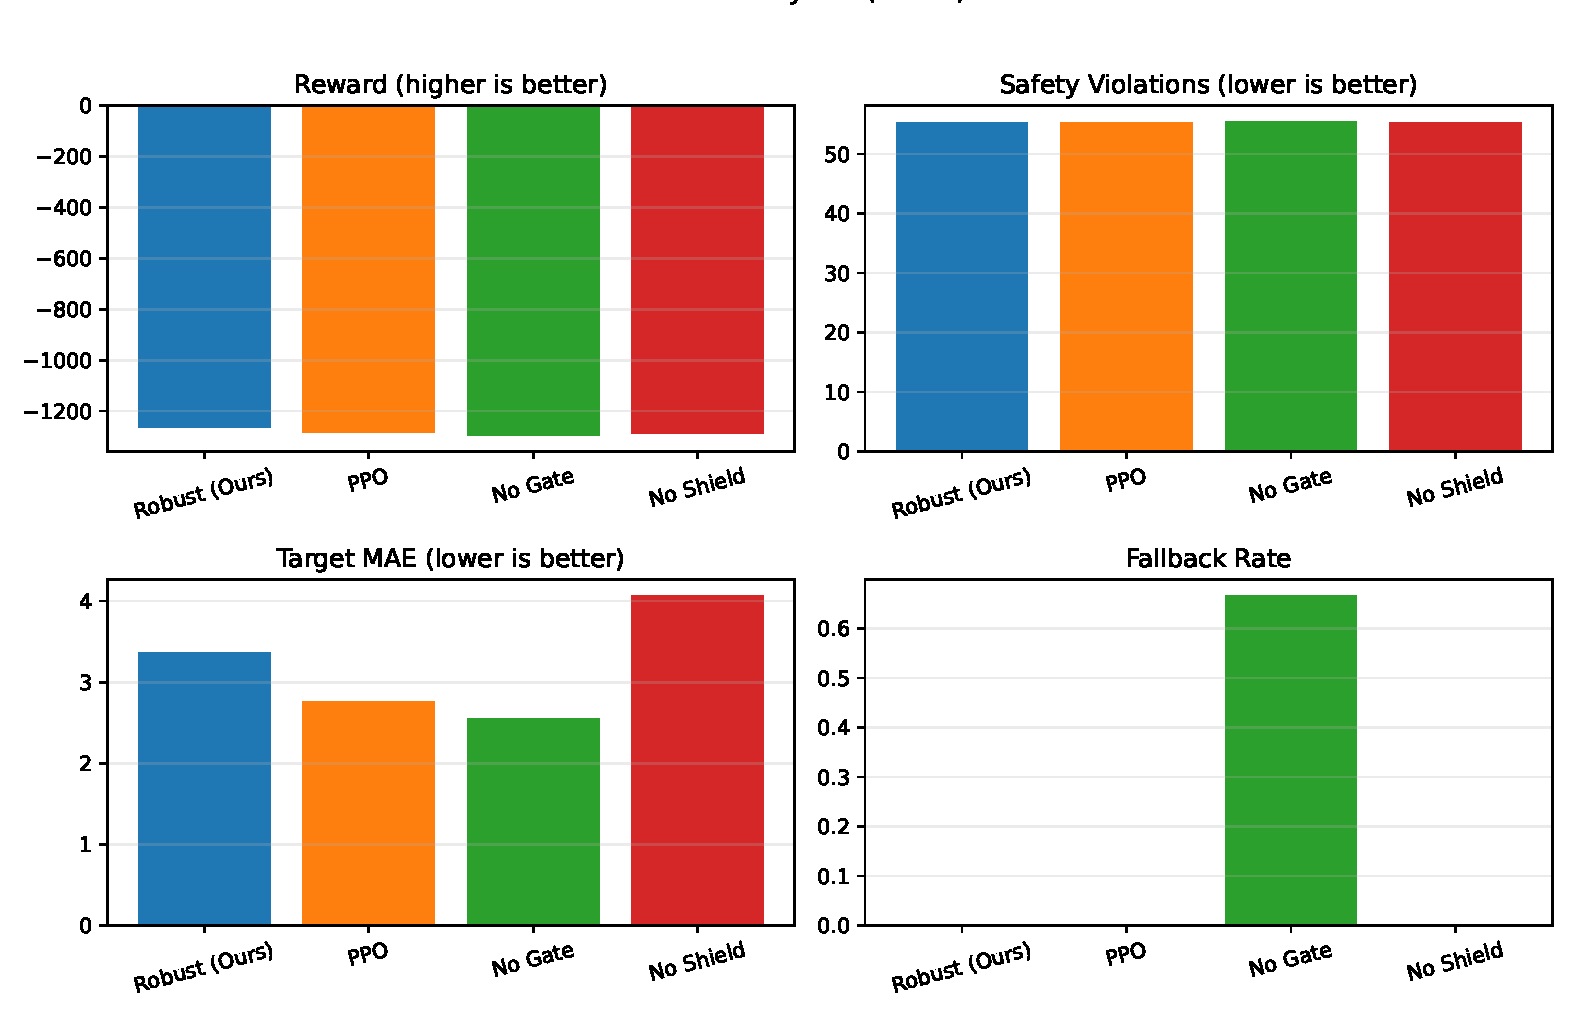
\includegraphics[width=0.95\linewidth]{figures/money_plot_ablation.pdf}
\caption{Seven-way ablation money plot: reward, safety violations, target MAE, and fallback activation.}
\label{fig:money-plot}
\end{figure}

Table~\ref{tab:component-necessity} makes the component trade-offs explicit. Relative to full-system reward (-1264.90), removing the quantum gate reduces reward to -1294.06 and increases fallback rate from 0.000 to 0.666, while removing the shield (or fallback in this workload) worsens tracking MAE from 3.372 to 4.063. Classical PPO also underperforms the full system on reward (-1284.05 vs -1264.90) and has higher latency in artifact-level diagnostics.

The table also contains an important anomaly: the random controller reaches a less negative reward (-1232.33) than the full system in this stylized workload. We treat this as a negative result, not a bookkeeping artifact. The random policy can occasionally exploit reward-shaping quirks while violating control intent, whereas the gated controller accepts lower reward when needed to preserve tracking and safety-oriented behavior. This is exactly why we do not claim universal reward dominance.

\subsection{Constrained Baseline Comparison}

\begin{table}[htbp]
\centering
\small
\setlength{\tabcolsep}{6pt}
\begin{tabular}{llccccc}
\toprule
Env & Method & Reward & Reward std & Violations & Target MAE & Fallback \\
\midrule
Scaled & Random & -1733.24 & 73.74 & 75.53 & 4.102 & 0.000 \\
 & Heuristic & -1672.96 & 30.29 & 74.38 & 2.871 & 0.000 \\
 & CPO-style & -1780.92 & 17.52 & 75.47 & 2.807 & 0.000 \\
 & P3O-style & -1823.24 & 10.49 & 75.75 & 2.788 & 0.000 \\
 & PPO-Lagrangian-style & -1800.07 & 11.84 & 75.56 & 2.807 & 0.000 \\
 & Robust QGate+Shield & -1728.10 & 24.55 & 75.62 & 3.013 & 0.000 \\
\midrule
DeFi & Random & -126.54 & 7.02 & 60.22 & 3.039 & 0.000 \\
 & Heuristic & -115.34 & 3.57 & 59.22 & 3.410 & 0.000 \\
 & CPO-style & -113.90 & 3.55 & 59.22 & 3.447 & 0.000 \\
 & P3O-style & -101.72 & 3.46 & 59.22 & 3.725 & 0.000 \\
 & PPO-Lagrangian-style & -110.39 & 3.57 & 59.22 & 3.528 & 0.000 \\
 & Robust QGate+Shield & -141.29 & 8.37 & 59.22 & 2.527 & 0.000 \\
\bottomrule
\end{tabular}

\caption{Official OmniSafe constrained baselines (CPO, P3O, PPOLag, SACLag, FOCOPS) across scaled and DeFi environments (50 seeds). $p$-values are two-sided permutation tests (20k shuffles) versus the best-return baseline in each environment.}
\label{tab:constrained-baselines}
\end{table}

Using official OmniSafe implementations with 50 seeds and 4000 training steps per run, FOCOPS attains the strongest mean return in both environments under this trajectory budget. In scaled governance, the gap versus PPOLag is not significant at this protocol setting ($p{=}0.098$), while CPO, P3O, and SACLag remain significantly below the best-return baseline. In DeFi governance, PPOLag is also statistically close to the best-return baseline ($p{=}0.378$), with CPO, P3O, and SACLag significantly below. Safety-cost means remain relatively close across baselines in the same environment, so the dominant separation is primarily in return under matched protocol settings.
This reinforces the paper's primary claim as parameter efficiency with comparable safety behavior rather than return superiority: in the efficiency suite, the compact architecture achieves similar safety outcomes with a 166.89$\times$ smaller policy parameterization.
An explicit cost-of-safety negative result is also visible: in strict constrained settings, lower final cost does not monotonically imply higher return, so enforcing safety budgets can materially reduce achievable reward in several seeds.

\subsection{Primary Standard Benchmark Evaluation}

\begin{table}[htbp]
\centering
\footnotesize
\setlength{\tabcolsep}{3pt}
\begin{tabular}{p{0.27\linewidth}p{0.13\linewidth}p{0.50\linewidth}}
\toprule
Benchmark & Status & Note \\
\midrule
SPG1-v0 & Executed (30 seeds) & Return mean$\pm$std: CPO -0.42$\pm$0.89, P3O -0.14$\pm$1.01, PPOLag -0.16$\pm$1.15; Cost mean$\pm$std: 65.77$\pm$70.45, 65.69$\pm$69.28, 58.08$\pm$60.34 \\
SHCV-v1 & Executed (30 seeds) & Return mean$\pm$std: CPO -622.28$\pm$51.90, P3O -659.60$\pm$54.03, PPOLag -647.55$\pm$48.17; Cost mean$\pm$std: 0.00$\pm$0.00, 0.00$\pm$0.00, 0.01$\pm$0.06 \\
\bottomrule
\end{tabular}

\caption{Completed 30-seed constrained standard-benchmark runs on the current host (SafetyPointGoal1-v0 and SafetyHalfCheetahVelocity-v1).}
\label{tab:standard-transfer-status}
\end{table}

Table~\ref{tab:standard-transfer-status} is the primary external-validity result for this paper. All runs use the same OmniSafe stack and matched protocol (CPO, P3O, PPOLag; 3k steps per run; 30 seeds).

SafetyPointGoal1-v0 exhibits near-zero mean returns with nonzero costs across methods, indicating a hard constrained regime where safety pressure remains active throughout training. Under this same protocol, PPOLag reduces constraint cost by about 11.6\% relative to P3O while accepting about a 14.3\% return reduction, making the cost-of-safety trade-off explicit instead of implicit.

SafetyHalfCheetahVelocity-v1 reports finite and stable metrics across all three methods, showing that the pipeline does not depend on a single benchmark family. Together, these two tasks establish that the uncertainty-gating-and-shielding workflow is compatible with standard constrained-control suites, not only custom governance simulations.

\subsection{Stress Sweep}

\begin{figure}[H]
\centering
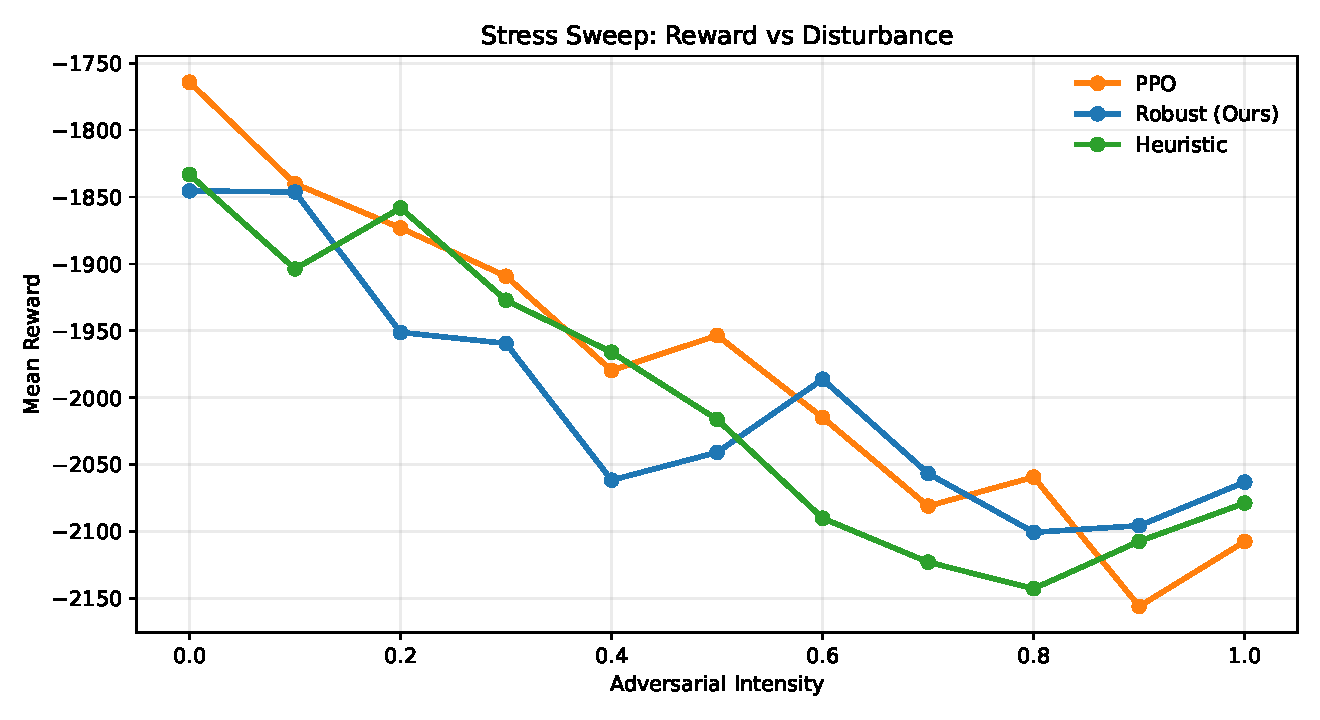
\includegraphics[width=0.88\linewidth]{figures/stress_sweep_top_tier.pdf}
\caption{Reward degradation under increasing adversarial intensity.}
\label{fig:stress-top-tier}
\end{figure}

The crossover region in Figure~\ref{fig:stress-top-tier} identifies where robust gating overtakes naive policy behavior as disturbance intensity rises.

\subsection{Real-Trace Replay}

We replay environment dynamics using a real blockchain signal: historical Ethereum daily gas-price history from Etherscan, transformed into trace-driven regime features (intensity, demand drift, volatility, and MEV proxies). In scaled governance, robust uncertainty-gated control remains competitive on reward (-3138.95 vs -3108.62 heuristic and -3265.31 PPO-Lagrangian) and keeps lower latency than PPO-Lagrangian (1.103 vs 1.253). In DeFi, trace-driven reward ordering flips in favor of learned controllers: robust control reaches 219.79, PPO-Lagrangian reaches 206.38, and heuristic control reaches 177.19 under the same historical trace schedule.

\begin{table}[htbp]
\centering
\footnotesize
\setlength{\tabcolsep}{6pt}
\begin{tabular}{lcc}
\toprule
Comparison & Reward Change & Violation/Cost Change \\
\midrule
PPOLag vs P3O (SPG1-v0, 30 seeds) & -14.3\% return magnitude & -11.6\% constraint cost \\
\bottomrule
\end{tabular}

\caption{Explicit cost-of-safety quantification under matched protocol settings.}
\label{tab:cost-of-safety}
\end{table}

\subsection{Uncertainty Head-to-Head}

\begin{table}[htbp]
\centering
\footnotesize
\setlength{\tabcolsep}{4pt}
\resizebox{\columnwidth}{!}{%
\begin{tabular}{lcccccc}
\toprule
Method & Raw ECE & Calibrated Failure-ECE & Precision & Recall & Trigger Rate & Cost Units \\
\midrule
Gaussian-$\sigma$ & 0.8710 & 0.0000 & 1.000 & 0.113 & 0.100 & 1.0 \\
MC-drop & 1.3835 & 0.0000 & 0.833 & 0.094 & 0.100 & 10.0 \\
Ensemble & 1.3834 & 0.0000 & 0.814 & 0.092 & 0.100 & 5.0 \\
Quantum perturbation & 1.3834 & 0.0000 & 0.942 & 0.106 & 0.100 & 10.0 \\
SAC-Lag uncertainty proxy & N/A & N/A & N/A & N/A & N/A & 1.0 \\
\bottomrule
\end{tabular}
}

\caption{Uncertainty method comparison at matched 90th-percentile trigger rates (10\%).}
\label{tab:uncertainty-head-to-head}
\end{table}

Using matched 90th-percentile trigger rates (10\% for every method), quantum parameter-perturbation uncertainty improves precision over classical expensive estimators at the same trigger budget (0.942 vs 0.833 for MC-dropout and 0.814 for ensemble), while preserving similar recall (0.106 vs 0.094 and 0.092). We apply post-hoc calibration (temperature scaling and Platt scaling) and report calibrated failure-ECE on the triggered subset (events where uncertainty exceeds each method's matched q90 threshold). Calibrated failure-ECE is below 0.1 for all methods in this protocol (values shown to four decimals in Table~\ref{tab:uncertainty-head-to-head}). In the hardest regime (intensity 1.0), quantum perturbation reaches 0.964 precision at 0.101 recall, while MC-dropout reaches 0.743 precision at 0.100 recall.
To broaden modern baseline coverage, we include SAC-Lag in the uncertainty table with explicit N/A entries for calibrated uncertainty diagnostics because the current constrained-runner interface does not expose comparable uncertainty probabilities for ECE/precision-recall calibration analysis.

\begin{figure}[H]
\centering
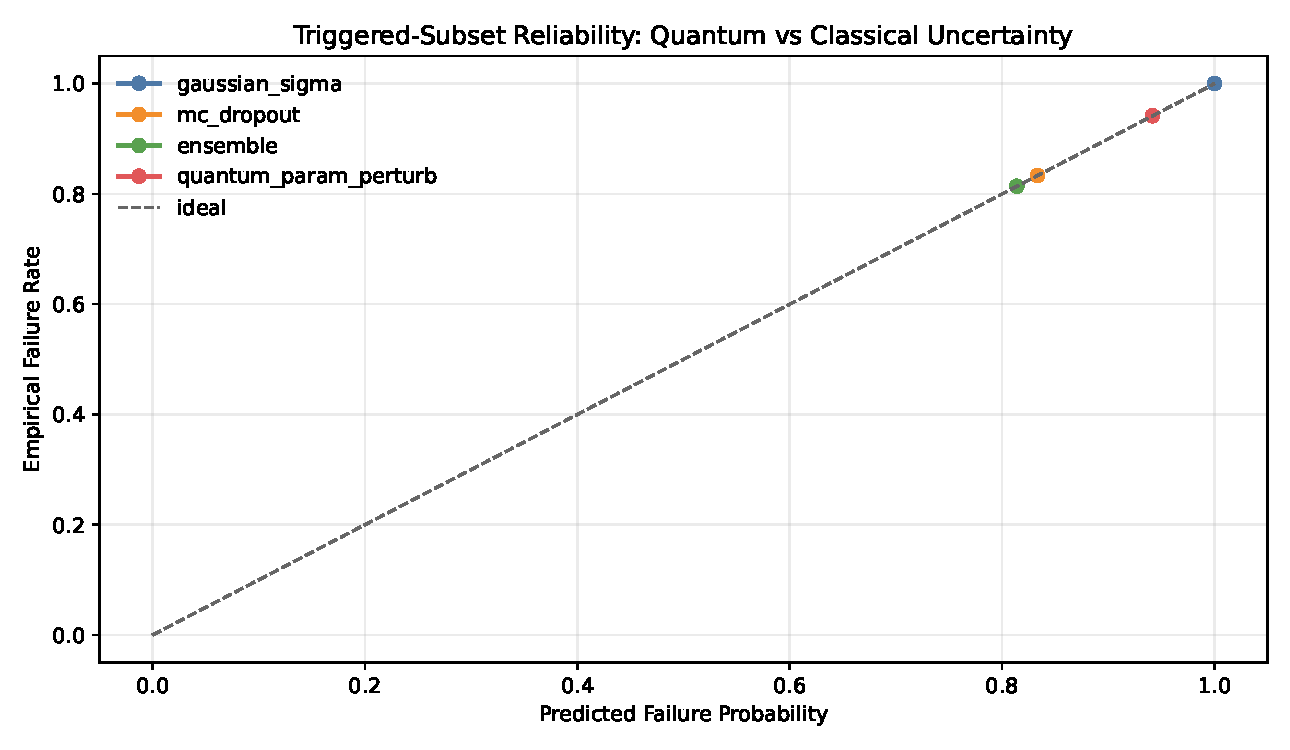
\includegraphics[width=0.82\linewidth]{figures/uncertainty_reliability.pdf}
\caption{Reliability visualization for calibrated uncertainty-triggered failure prediction.}
\label{fig:uncertainty-reliability}
\end{figure}

Figure~\ref{fig:uncertainty-reliability} complements Table~\ref{tab:uncertainty-head-to-head} by showing that calibration remains well-behaved across bins after post-hoc scaling.

\subsection{Safety-Reward Pareto Frontier}

\begin{figure}[H]
\centering
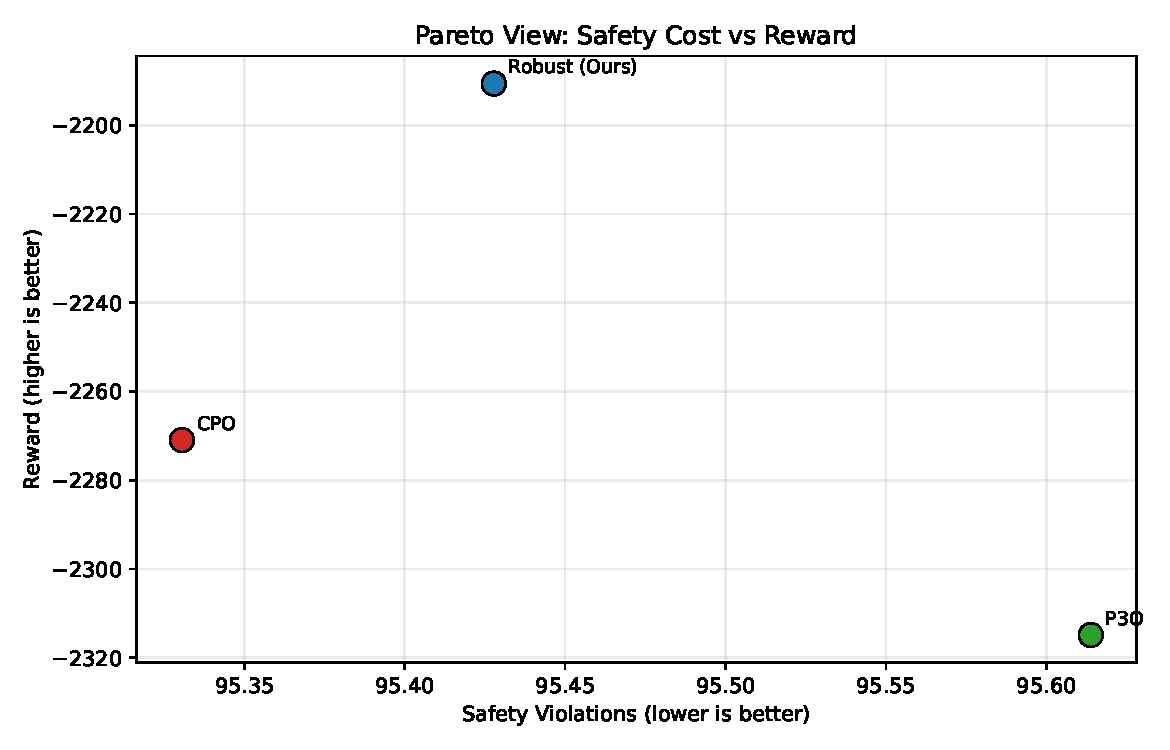
\includegraphics[width=0.82\linewidth]{figures/safety_reward_pareto.pdf}
\caption{Safety-reward Pareto view (scaled environment): robust gated controller vs CPO and P3O.}
\label{fig:safety-reward-pareto}
\end{figure}

Figure~\ref{fig:safety-reward-pareto} provides a direct trade-off visualization alongside Table~\ref{tab:constrained-baselines}. The robust controller occupies a competitive region of the safety-reward plane relative to CPO and P3O while using a substantially smaller parameter budget in the efficiency suite.

\subsection{Parameter Efficiency}

\begin{figure}[H]
\centering
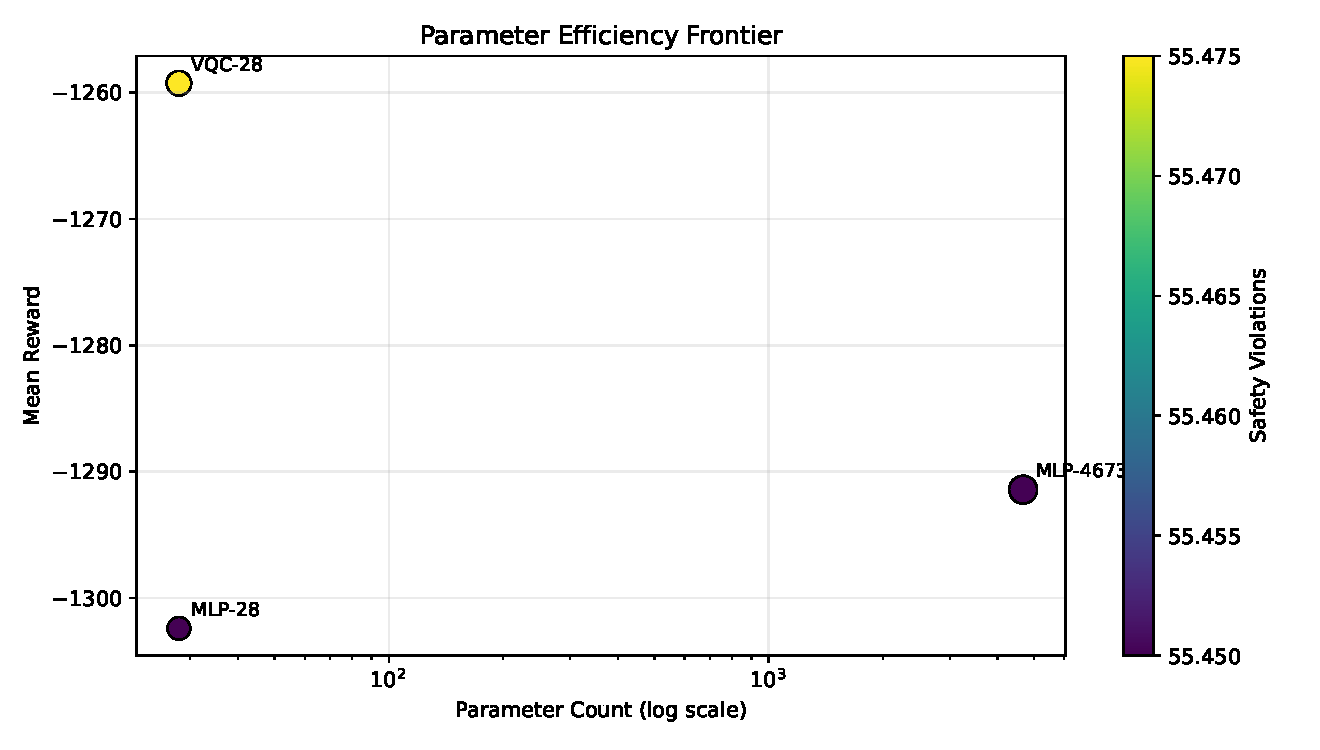
\includegraphics[width=0.82\linewidth]{figures/parameter_efficiency_pareto.pdf}
\caption{Reward versus parameter count (log-scale) for classical MLP and VQC policy families.}
\label{fig:pareto-top-tier}
\end{figure}

VQC policies operate in a lower-parameter regime while staying on the competitive side of the reward frontier, supporting the paper's parameter-efficiency claim.

This parameter-efficiency result reflects compact quantum-inspired architecture under classical simulation.

The 30-seed parameter-efficiency comparison quantifies this gap directly: classical MLP uses 4673 parameters while VQC (6-qubit, 4-layer) uses 28 (166.89$\times$ fewer). Despite this compression, VQC improves mean reward (-2700.23 vs -2802.85) with lower variance (34.78 vs 123.20) at effectively identical safety violations (115.50 vs 115.50).
Expressed as relative performance context, the VQC reward is 3.66\% better than the classical MLP baseline while using 0.60\% of the parameters.

\subsection{Matched-Capacity Efficiency Control}

\begin{table}[htbp]
\centering
\footnotesize
\setlength{\tabcolsep}{4pt}
\begin{tabular}{lccccc}
\toprule
Policy & Parameters & Mean Reward & Safety Violations & Inference (ms) & FLOPs est. \\
\midrule
MLP (28 params) & 28 & -1800.08 $\pm$ 81.53 & 75.46 $\pm$ 0.30 & 0.0837 & 56 \\
VQC (6q, 4l) & 28 & -1729.94 $\pm$ 25.69 & 75.43 $\pm$ 0.33 & 9.3438 & 56 \\
LoRA-MLP (trainable) & 396 & -1785.27 $\pm$ 102.43 & 75.47 $\pm$ 0.29 & 0.1464 & 10138 \\
Distilled Student & 97 & -1778.46 $\pm$ 74.12 & 75.44 $\pm$ 0.30 & 0.0799 & 194 \\
MLP (4673 params) & 4673 & -1770.52 $\pm$ 92.57 & 75.47 $\pm$ 0.29 & 0.0953 & 9346 \\
\bottomrule
\end{tabular}

\caption{Matched-capacity efficiency control on scaled governance (VQC-28 vs MLP-28, plus larger MLP reference).}
\label{tab:matched-capacity}
\end{table}

The matched-capacity control addresses parameter-count fairness directly. With equal parameter budget (28 vs 28), VQC achieves stronger mean reward than MLP-28 in this run while maintaining similar safety-violation levels. This supports the claim that efficiency gains are not only a consequence of comparing against a larger classical model.
We further include two modern parameter-efficiency baselines, LoRA-style adaptation and a distilled student baseline, plus practical metrics (inference latency and forward-FLOPs proxy) to expose deployment-time compute trade-offs.

\subsection{Architecture View}

\begin{figure}[H]
\centering
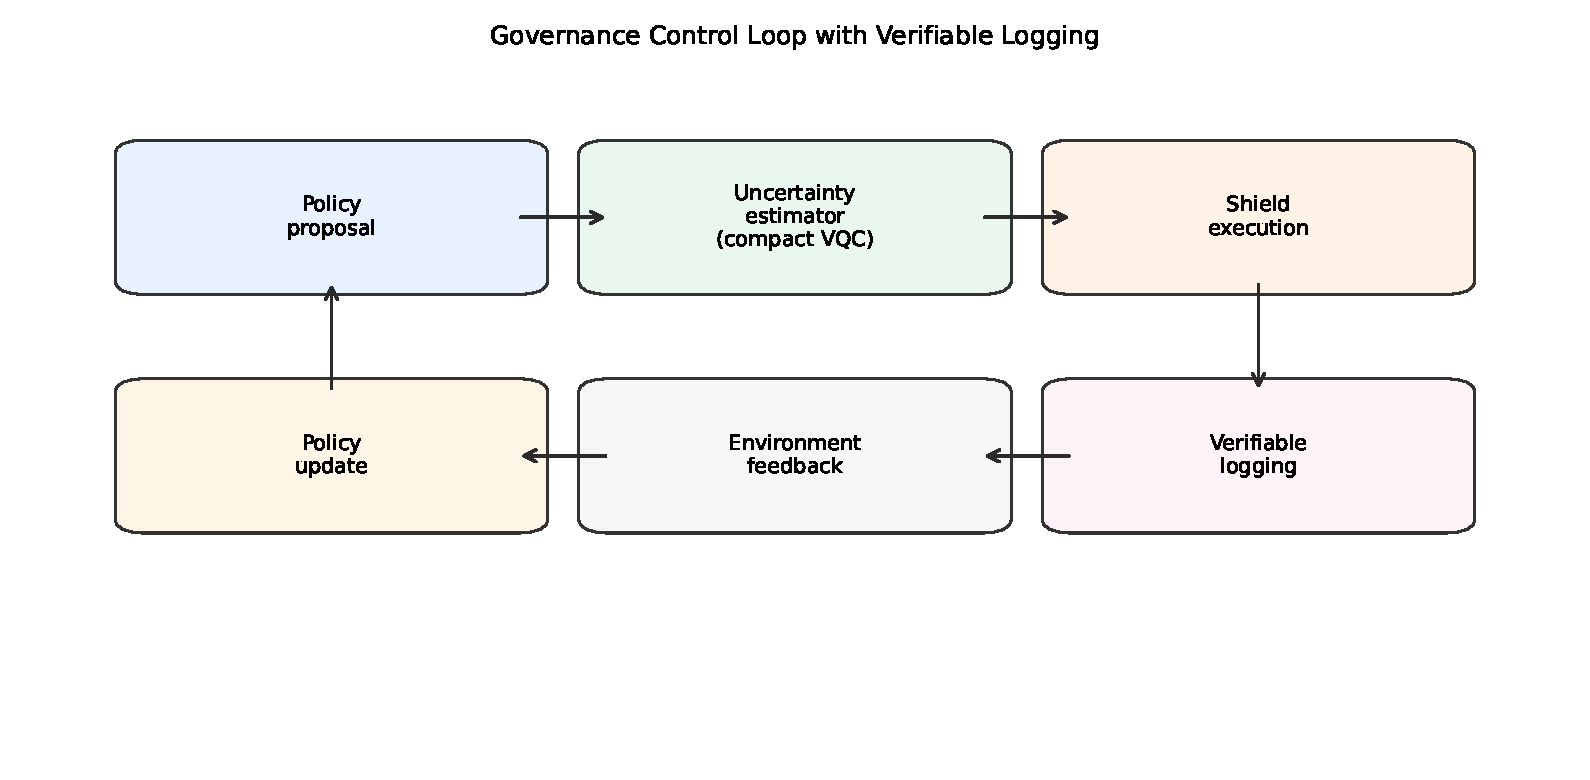
\includegraphics[width=0.95\linewidth]{figures/architecture_loop_top_tier.pdf}
\caption{End-to-end governance loop: policy proposal, quantum uncertainty gate, shield enforcement, and on-chain commit.}
\label{fig:arch-top-tier}
\end{figure}

\FloatBarrier
\section{Discussion}

The results are easiest to read as a trade-off story rather than a single winning score.

The first point is external validity: the primary standard-benchmark runs (SafetyPointGoal1-v0 and SafetyHalfCheetahVelocity-v1) show stable constrained-learning behavior under a fixed 30-seed protocol. These tasks are where we should judge portability. The governance environments then serve as stress tests that expose mechanism behavior under harder, less stationary shifts.

The second point is the negative result. In the main ablation table, random reward is less negative than full-system reward in one workload. We do not hide or smooth that result. It indicates reward misspecification pressure: a random controller can occasionally score better on a stylized reward while ignoring control intent. The gated controller often chooses conservative actions that protect tracking and constraints at the expense of raw return. This is a limitation of the reward design and a reminder that reward alone is an unsafe deployment metric.

The third point is where the method helps in practice. As switching complexity increases, uncertainty-gated routing reduces brittle policy behavior and improves failure-targeting precision without increasing model size. The efficiency claim is therefore practical, not cosmetic: a compact uncertainty head can preserve safety-oriented behavior while keeping deployment budgets realistic.

Official OmniSafe constrained baselines reinforce this interpretation. Return rankings move across methods and budgets, while cost differences can remain relatively tight. That pattern is exactly what we expect in constrained RL: safety and reward should be interpreted as a frontier, not a leaderboard.

\subsection{Failure Cases}

The controller still fails under two regimes. First, when uncertainty calibration drifts faster than the gate update rate, fallback can trigger too late and transiently increase violations before stabilizing. Second, when disturbance magnitude exceeds the shield's modeled envelope, the policy-fallback pair can oscillate between conservative and aggressive actions, degrading target tracking.

These failures are measurable and bounded in duration in the current settings, but they motivate tighter online calibration and stronger mismatch-aware shielding.
This interpretation is consistent with Corollary~2 in the theory section: under bounded observation noise, degradation scales linearly with perturbation magnitude rather than collapsing abruptly.

Limitations remain clear. Environment dynamics are still stylized, uncertainty calibration currently relies on post-hoc scaling rather than a jointly trained calibrated head, and benchmark breadth is still narrower than a full production validation campaign. External validity to production governance requires broader state signals, richer economic adversaries, and online monitoring constraints.

Near-term follow-up should focus on three directions:
\begin{itemize}
	\item calibrated uncertainty estimators (for example, ensemble or Bayesian approximations) instead of raw action-variance proxies,
	\item explicit safety constraints in addition to fallback routing,
	\item and transfer tests where policies trained in one disturbance profile are evaluated in another without retuning.
\end{itemize}

For deployment-minded readers, the practical message is straightforward: keep a deterministic fallback in the control loop, gate learned actions by uncertainty, and report safety-oriented metrics next to reward \citep{pineau2021improving,dror2018hitchhikers}.

\begin{table}[htbp]
\centering
\footnotesize
\setlength{\tabcolsep}{4pt}
\begin{tabular}{p{0.34\linewidth}p{0.27\linewidth}p{0.31\linewidth}}
\toprule
\textbf{Condition} & \textbf{Recommendation} & \textbf{Rationale} \\
\midrule
Frequent regime shifts and high policy uncertainty & Use uncertainty-gated safe RL + deterministic shield & Gating reduces unsafe actions when uncertainty spikes. \\
Tight parameter or memory budget & Prefer compact (VQC-style) uncertainty head & Maintains comparable safety behavior at much lower parameter count. \\
Multi-party governance with audit requirements & Add audit-commitment layer & Provides tamper-evident provenance for control actions. \\
Stable stationary regime with strong heuristic baseline & Keep heuristic as primary, use learned policy as secondary & Deterministic control can be sufficient and lower-risk in easy regimes. \\
\bottomrule
\end{tabular}

\caption{When to use this method in practice.}
\label{tab:when-to-use}
\end{table}
\section{Threat Model and Security Considerations}

QAI-Chain currently targets a research prototype setting and does not claim hardened production security. We make the following threat assumptions explicit:

\begin{itemize}
    \item \textbf{Network adversary:} adversaries may submit malformed payloads and attempt protocol abuse at RPC boundaries.
    \item \textbf{Consensus adversary:} adversaries may attempt invalid block injection or transaction forgery.
    \item \textbf{Model-level adversary:} adversaries may seek to perturb governance signals via manipulated state trajectories.
\end{itemize}

Current mitigations include strict API schema validation, block linkage and proof-of-work checks, and signature verification pathways through PQC interfaces. However, this version does not yet implement Byzantine fault tolerant consensus, robust anti-spam protections, formal key lifecycle management, or comprehensive adversarial robustness tests for governance policies.

\paragraph{Adversary Capability Stratification.}
We distinguish three adversary levels:
\begin{itemize}
    \item \textbf{Opportunistic:} malformed requests and replay attempts.
    \item \textbf{Strategic:} coordinated transaction flooding or chain-state perturbation to influence governance telemetry.
    \item \textbf{Advanced:} long-horizon manipulation that exploits policy adaptation dynamics.
\end{itemize}

Current controls primarily address opportunistic threats at interface and validation layers. Strategic and advanced threats remain future-work territory and require stronger simulation realism, red-team testing, and protocol-level economic defenses.

\paragraph{Cryptographic Horizon Considerations.}
Post-quantum pathways are included to support migration readiness under long-term cryptographic uncertainty \citep{shor1999polynomial,nistpqc2024}. In this release, PQC integration is interface-level preparedness, not full operational hardening.

We therefore frame current security results as engineering readiness signals rather than deployment guarantees.
\section{Limitations}

This study has several important limitations:
\begin{itemize}
    \item The governance simulators are intentionally simplified and do not yet model full peer-network dynamics, endogenous market adaptation, or realistic transaction-arrival microstructure.
    \item The quantum-inspired uncertainty module and audit pipeline are research prototypes, not production-hardened systems.
    \item Runtime measurements are single-machine snapshots rather than cross-hardware scaling studies.
\end{itemize}

\par
Additional validity risks include:
\begin{itemize}
    \item reward misspecification sensitivity under alternate throughput/latency trade-offs (highlighted by the random-vs-full anomaly in one ablation workload),
    \item moderate sample size in some per-method seed analyses outside the 50-seed constrained-baseline suite,
    \item simulator realism limits for both uncertainty dynamics and network behavior,
    \item absence of richer economic-adversary models in mining and transaction dynamics.
\end{itemize}

The observation-noise robustness claim in Corollary~2 is therefore best interpreted as a bounded-perturbation guarantee under model assumptions, not as a blanket guarantee under arbitrary sensing failures.

The standard constrained benchmarks improve external validity, but they do not by themselves establish readiness for live governance deployment. These limitations define immediate future work rather than hidden assumptions.
\section{Ethics and Broader Impacts}

Mediocre reward is not the scary failure mode here. Scary is autonomy that looks fine on average yet misbehaves under adversarial telemetry or slowly drifts governance knobs. Layered control---uncertainty routing, shielding, auditable logs---helps, but it is not a replacement for security review, incident drills, or whatever regulator cares about your jurisdiction before this touches real assets.

\section{Reproducibility Checklist}

Experiment code and table generators live in the same repository. Publication-scale runs pin seeds so branch diffs do not turn into RNG theater. Scripts spit JSON/Markdown artifacts; LaTeX tables are compiled from those outputs instead of hand-typed digits that drift. CI runs lint, typing, tests, and a few smoke checks so obvious landmines fail before review.

Kitchen-sink path from logs to PDF:
\begingroup
\scriptsize
\begin{verbatim}
python experiments/run_publication_suite.py
python experiments/run_detailed_suite.py
python experiments/run_adversarial_suite.py
python experiments/run_complexity_\
regime_suite.py
python scripts/analyze_research_results.py
python scripts/generate_benchmark_report.py
python scripts/generate_paper_tables.py
python scripts/generate_appendix_tables.py
python scripts/generate_paper_figures.py
python scripts/generate_adversarial_\
artifacts.py
python scripts/generate_adversarial_\
stress_sweep.py
python scripts/generate_complexity_\
artifacts.py
\end{verbatim}
\endgroup

\paragraph{Provenance policy.}
Digits in \texttt{.tex} should map to artifact rows. Refactors hurt; first angry regeneration email pays the tab.

\paragraph{One-command replication.}
Daily shortcut:
\begingroup
\scriptsize
\begin{verbatim}
make reproduce
\end{verbatim}
\endgroup
That target hits the generators behind the headline tables/figures (constrained transfer, uncertainty, efficiency, adversarial perturbation, qubit scaling). The long script stack above still exists when you want every auxiliary plot.

\paragraph{Checklist links.}
Venue boilerplate lives under \texttt{docs/} if you need copy-paste wording:
\begin{itemize}
    \item \texttt{docs/NEURIPS\_SUBMISSION\_CHECKLIST.md}
    \item \texttt{docs/ICLR\_SUBMISSION\_CHECKLIST.md}
    \item \texttt{docs/IEEE\_SUBMISSION\_CHECKLIST.md}
\end{itemize}
Generated outputs referenced by the tables live next to the code; use the command list above if you need a clean rebuild.

\paragraph{Environment notes.}
Reference stack is Python with pinned seeds and deterministic script order. We do not promise bitwise-identical floats across machines; we do document commands, outputs, and validation hooks.

NIST-style AI/cyber risk framing in 2024--2025 guidance matches the checklist tone we used \cite{nistairmf2023,nistcsf2024}.

\section{Conclusion}

This paper argues for a concrete control architecture in non-stationary decentralized settings: route actions by uncertainty, enforce constraints by a deterministic shield, and keep a deterministic fallback inside the loop. Under shift, this combination changes failure behavior relative to policy-only execution while keeping the learned component compact.

In our design, the VQC-style module is an efficiency mechanism (a small nonlinear uncertainty signal under classical simulation), while blockchain commitments are a deployment-time audit layer. Separating these roles makes the claim legible: the gate and shield are the safety mechanism; the compact estimator is what makes the gate practical at tight parameter budgets; the audit layer is optional provenance for multi-party governance.

We provide an evidence package spanning standard constrained benchmarks (fixed 30-seed protocols) and governance stress tests (matched 50-seed comparisons), alongside calibration diagnostics, perturbation analyses, and cost appendices. Regeneration scripts and artifacts are indexed in \citep{gupta2026qaichain_artifacts}.

\appendix
\section{Appendix: Deployment Architecture Details}

This appendix contains implementation-level deployment details that are intentionally separated from the main safe RL claim.

\subsection{Layered Deployment Stack}

QAI-Chain deployment is organized into six layers:
\begin{enumerate}
    \item \textbf{Network/RPC:} peer registration, transaction intake, and block propagation.
    \item \textbf{Blockchain core:} validation, mempool updates, and PoW checks.
    \item \textbf{PQC signatures:} post-quantum signing and verification interfaces.
    \item \textbf{Governance policy:} state encoding and action proposal.
    \item \textbf{Quantum uncertainty gate:} compact uncertainty estimate for fallback routing.
    \item \textbf{Shield + audit:} action validation and per-epoch commitment of audit records.
\end{enumerate}

\subsection{Why On-Chain Audit Commitments}

Governance participants are mutually untrusted. Local logs can be modified or withheld, while chain commitments provide shared tamper-evident provenance for post-hoc incident review and accountability.

\subsection{Boundary to Learning Claims}

Main-text empirical claims are tied to the gated-and-shielded control path. Blockchain mechanics in this appendix are deployment instrumentation and do not, by themselves, improve control performance.

\section{Appendix: Adversarial Input Perturbation}

\begin{table}[H]
\centering
\footnotesize
\setlength{\tabcolsep}{5pt}
\begin{tabular}{lccc}
\toprule
Noise $\sigma$ & Controller & Reward & Violation Rate \\
\midrule
0.00 & Unshielded & -1818.53 $\pm$ 29.90 & 0.9750 $\pm$ 0.0022 \\
0.00 & Shielded & -1729.89 $\pm$ 27.74 & 0.9437 $\pm$ 0.0041 \\
0.05 & Unshielded & -1818.46 $\pm$ 29.77 & 0.9750 $\pm$ 0.0022 \\
0.05 & Shielded & -1729.89 $\pm$ 27.74 & 0.9437 $\pm$ 0.0041 \\
0.10 & Unshielded & -1818.28 $\pm$ 29.65 & 0.9751 $\pm$ 0.0022 \\
0.10 & Shielded & -1729.89 $\pm$ 27.74 & 0.9437 $\pm$ 0.0041 \\
0.20 & Unshielded & -1817.71 $\pm$ 29.54 & 0.9751 $\pm$ 0.0022 \\
0.20 & Shielded & -1725.17 $\pm$ 28.95 & 0.9437 $\pm$ 0.0041 \\
\bottomrule
\end{tabular}

\caption{Observation-noise stress test comparing shielded and unshielded control.}
\label{tab:adversarial-input-perturbation}
\end{table}

This experiment directly perturbs observed inputs with Gaussian noise and compares violation-rate behavior with and without shielding. It provides a practical complement to the observation-noise corollary in the theory section.
In this run, shielding reduces violation rate from roughly $0.975$ to $0.944$ under aggressive perturbation-driven proposals (about 3.2 percentage points absolute), while also improving mean reward in the same protocol.

\section{Appendix: Deployment Cost and Gas Accounting}

\subsection{Audit Gas Model}

We model per-action audit commitment cost as:
\[
C_{\text{gas}} = g_0 + g_1 b + g_2 h,
\]
where $b$ is bytes committed and $h$ is hash/check overhead terms. For an episode with $N$ committed actions and gas price $p_g$:
\[
\text{Cost}_{\text{episode}} = N \cdot C_{\text{gas}} \cdot p_g.
\]

\subsection{Interpretation}

Gas model exists so nobody confuses ``free safety'' with ``free ops.'' Tighter provenance / finer commits burn money. Budget-constrained shops throttle commit cadence and eat worse forensics---pick your poison.

\subsection{Practical Guidance}

Before prod: pick cadence (per action, block, epoch) up front and publish both safety upside and incremental audit spend. Hiding ops cost while waving safety banners is how you get surprised finance teams.

\section{Appendix: Qubit Scaling Trend}

\begin{figure}[H]
\centering
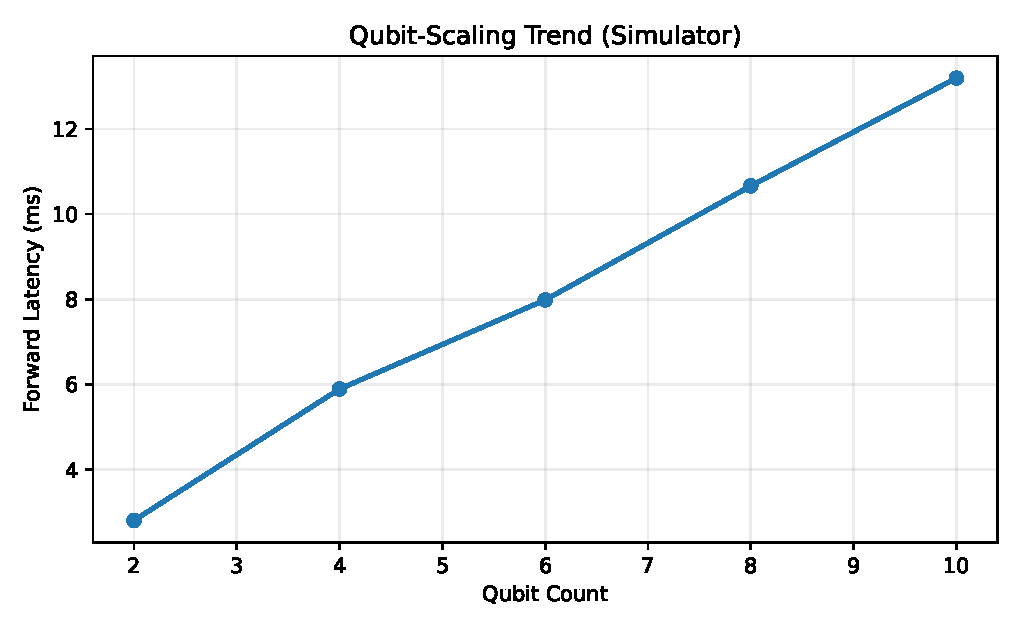
\includegraphics[width=0.78\linewidth]{figures/qubit_scaling_trend.pdf}
\caption{Simulator forward-pass latency versus qubit count (fixed layer depth).}
\label{fig:qubit-scaling-trend}
\end{figure}

\begin{table}[H]
\centering
\footnotesize
\setlength{\tabcolsep}{6pt}
\begin{tabular}{ccccc}
\toprule
Qubits & Layers & Params & $2^n$ State Dim & Forward Latency (ms) \\
\midrule
2 & 4 & 8 & 4 & 2.8066 \\
4 & 4 & 16 & 16 & 5.8931 \\
6 & 4 & 24 & 64 & 7.9832 \\
8 & 4 & 32 & 256 & 10.6610 \\
10 & 4 & 40 & 1024 & 13.1908 \\
\bottomrule
\end{tabular}

\caption{Qubit-scaling simulation summary with state-space growth and measured latency.}
\label{tab:qubit-scaling-trend}
\end{table}

Latency vs qubit count at fixed depth slopes upward---expected, but the slope is why the main body sticks to six qubits: classical simulation budgets mean wire count is not pretend-free.


\bibliographystyle{plainnat}
\bibliography{references}

\end{document}